% $Header: /cvsroot/latex-beamer/latex-beamer/solutions/conference-talks/conference-ornate-20min.de.tex,v 1.7 2004/10/07 20:53:08 tantau Exp $

\documentclass{beamer}

\mode<presentation>
{
  	\usetheme{Frankfurt}
  	\usecolortheme{seahorse}
	\useinnertheme{circles}  

  \setbeamercovered{transparent}
  % oder auch nicht
}

\usepackage{color}
\usepackage{graphicx}
\usepackage{epstopdf}


\usepackage[german]{babel}
% oder was auch immer

\usepackage[utf8]{inputenc}
% oder was auch immer

\usepackage{times}
\usepackage[T1]{fontenc}
% Oder was auch immer. Zu beachten ist, das Font und Encoding passen
% mssen. Falls T1 nicht funktioniert, kann man versuchen, die Zeile
% mit fontenc zu lschen.


\title[Pflichtenheft] % (optional, nur bei langen Titeln ntig)
{e-puck Conquest}

\subtitle
{Pflichtenheft}

\author[Autor, Anders] % (optional, nur bei vielen Autoren)
{SEP - ITS 2010 \\ Max Binder \and Florian Bürchner \and Martin Freund
	\\ Florian Lorenz \and Andreas Poxrucker \and Andreas Wilhelm}
% - Namen mssen in derselben Reihenfolge wie im Papier erscheinen.
% - Der \inst{?} Befehl sollte nur verwendet werden, wenn die Autoren
%   unterschiedlichen Instituten angehren.

\institute[Universität Passau] % (optional, aber oft ntig)
{
  Fakultät für Informatik und Mathematik\\
  Universität Passau}

\AtBeginSubsection[]
{
  \begin{frame}<beamer>
    \frametitle{Gliederung}
    \tableofcontents[currentsection,currentsubsection]
  \end{frame}
}


% Falls Aufzhlungen immer schrittweise gezeigt werden sollen, kann
% folgendes Kommando benutzt werden:

%\beamerdefaultoverlayspecification{<+->}



\begin{document}

\begin{frame}
  \titlepage
\end{frame}

\begin{frame}
  \frametitle{Gliederung}
  \tableofcontents
  % Die Option [pausesections] knnte ntzlich sein.
\end{frame}

\section{Einleitung}

\begin{frame}
  \frametitle{Motivation}

	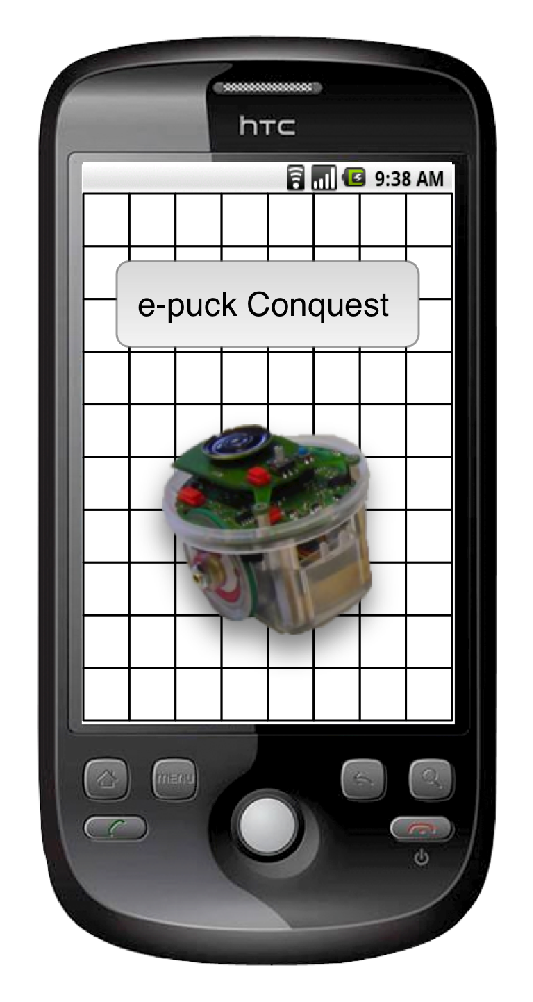
\includegraphics[height=5cm]{logo.eps} 
	\begin{itemize}
		\item Aufgabenstellung
		\item 
	\end{itemize}
\end{frame}

\begin{frame}
  \frametitle{Anwendungsbereiche}

Mögliche Anwendungen sowie Erweiterungen unseres Systems sind:

	\begin{itemize}
	    \item	Vermessung von Baugebieten
        Putzroboter für dein Einsatz im Alltag
	•	Grundsrisszeichnungen für neue Wohnungen
	•	Systematisches Absuchen von Gebieten (Wald, Wohnungsboden)	
	\end{itemize}

\end{frame}

\section{Aufgabenstellung}

\begin{frame}
  \frametitle{Musskritierien aus dem Lastenheft}
  
	\begin{itemize}
	•	Erkundung von unbekannten Spielfeldern
	•	Kommunikation und Kooperation der e-puck Roboter ohne zentrale Steuereinheit (Master/Slave)
	•	Darstellung der bereits erkundeten Karte auf dem Smartphone sowie die aktuelle Position der Roboter
	•	Auswahl und Steuerung eines einzelnen e-puck Roboters
	\end{itemize}  
\end{frame}

\begin{frame}
  \frametitle{Pflichtenheft}
  
  	\begin{itemize}
	•	Genaue Rahmenbedingungen für das Spielfeld (Größe von Quadraten usw.)
	•	Festedefinierte Startplätze
	•	Feldgröße von mindestens 10cm x 10cm
	•	Kollisionserkennung und Vermeidung
	\end{itemize}  
\end{frame}

\begin{frame}
  \frametitle{Wunschkriterien}
  
  	\begin{itemize}
	•	Zustandvisualisierung
	•	Bel. Startpositionen
	•	Exportfunktion für die Karte
	•	Pfadanzeige der einzelnen Roboter
	\end{itemize}  
\end{frame}


\section{Abgrenzungskriterien}

\begin{frame}
  \frametitle{berschriften mssen informativ sein.}
\end{frame}

\begin{frame}
  \frametitle{berschriften mssen informativ sein.}
\end{frame}

\begin{frame}
  \frametitle{berschriften mssen informativ sein.}
\end{frame}



% Alles nachfolgende ist optional und typischerweise nicht ntig.
\appendix
\section<presentation>*{\appendixname}
\subsection<presentation>*{Weiterfhrende Literatur}

\begin{frame}[allowframebreaks]
  \frametitle<presentation>{Weiterfhrende Literatur}
    
  \begin{thebibliography}{10}
    
  \beamertemplatebookbibitems
  % Anfangen sollte man mit bersichtswerken.

  \bibitem{Autor1990}
    A.~Autor.
    \newblock {\em Einfhrung in das Prsentationswesen}.
    \newblock Klein-Verlag, 1990.

    
  \beamertemplatearticlebibitems
  % Vertiefende Literatur kommt spter. Die Liste sollte kurz sein.

  \bibitem{Jemand2000}
    S.~Jemand.
    \newblock On this and that.
    \newblock {\em Journal of This and That}, 2(1):50--100, 2000.
  \end{thebibliography}
\end{frame}

\end{document}


